\chapter{Evaluation}\label{chapter:Evaluation}


\section{Accessibility}
In order to provide a comprehensive analysis of the accessibility violations, 
we divide the analysis into 3 categories. Those categories differentiate in 
terms of quantitive and qualitive analysis as well as in its depth.

\subsection{Quantitive Analysis}
Figure x shows the quantitive analysis of the amount and type of Accessibility 
Violations found during the 3 experiment runs for each tuple of parameters.
Based on this figure, we can observe several interesting findings.\newline
Firstly, the amount and types of Accessibility Violations show a similar 
patterns across the different models. While overall \textit{gpt-4o} produced
slightly less violations, its numbers and distribution show a similar 
structure. 
Without the refinement techniques, we also see a very skewed error profile. 
Color contrast violations, as well as HTML landmark and region 
issues are the predominantly cause for at least 75\% of all violations in both
gemini's flash-2.5 and in gpt-4o model and with diverse prompting techniques.\newline
While gemini seems to have more color contrast violations, 
landmark and region rules cause more problems for the gpt-4o model. Those 
findings are confirmed across different parameters.\newline
The subsequent types of violations are in the fields of missing labels,
links without distinguishable color, issues with the HTML header and 
the size of frontend components. The results show a noticeable trend that 
only a small subset of possible WCAG violations cause non-negligible amounts 
of violations in an Image-to-Code environment. Especially in the case of 
gpt-4o, there are only 6 types of violations which cause more than 10
violations combined across all prompting techniques in our dataset.\newline
Similar to related papers in this field (paper xxx), our results also show 
that different prompting techniques only have small impact on the findings.
Even if the naive prompting approach does not instruct the LLMs to generate
code with compliance to the WCAG standards, it still only shows slightly 
increased amounts of violations than more advanced prompting techniques such as 
zero-shot or reasoning.\newline
Figure xyy shows the violations found in the ground truth HTML/CSS of our 
dataset. The human-written HTML/CSS of our dataset counts 1339 accessibility 
violations, leading to $\sim$25.26 violations per file across the whole dataset.
On the other hand, even gemini with the naive prompting technique,
the worst performing set of parameter, had a maximum of 917 accessibility 
violations, leading to $\sim$17.3 violations per file across the whole dataset.
This shows that LLMs write by default more accessible code than humans by 
incorporating the most important rules. However, as described above they 
struggle with more complex rules such as color contrast or landmarks
that require further information or thinking.

IR noch mit aufnehmen.
IW-IR noch mit aufnehmen.
Verteilung der Issues bei Human und LLms mit aufnehmen.
Bar Charts noch mit aufnehmen ohne iterative


\subsection{Qualitive Analysis}
In a first step, we analyze how consistent violations are within different 
within different experiment runs and dataset entries. Figure xy shows the 
consistency of the type and the amount of a violation by using the 
\textit{cosine-similarity}. Therefore, we analyze the type of violation
and its amount per file in vector-like structure. 
The cosine-similarity is then calculated between the vectors of the 
different experiment runs and dataset entries. This allows us to 
analyze how similar the violations are and to understand how consistent
the LLMs are in generating accessible code.

\newcommand{\vect}[1]{\begin{pmatrix}#1\end{pmatrix}}
\newcommand{\issues}{k}                   % Anzahl der Issue-Klassen
\newcommand{\vx}{\mathbf x}
\newcommand{\vy}{\mathbf y}

\begin{enumerate}
  \item \textbf{Amount of Issues}  
        For each test run and file we are counting the number of violations per class
        \[
          \left(
            \begin{array}{@{}l r@{}}
              \text{Issue}_{1}: & x_{1}\\
              \text{Issue}_{2}: & x_{2}\\
              \vdots           & \vdots\\
              \text{Issue}_{\issues}: & x_{\issues}
            \end{array}
          \right)
          \xmapsto{\text{to vector}}
          \vx \;:=\;
          \vect{x_{1}\\x_{2}\\\vdots\\x_{\issues}} \in \mathbb R^{\issues}.
        \]

  \item \textbf{Calculation of Cosine Similarity}  
        Given two experiment runs with $\vx,\vy\in\mathbb R^{\issues}$, we define
        \[
          \operatorname{cos\_sim}(\vx,\vy)=
          \frac{\vx^{\mathsf T}\vy}{\lVert\vx\rVert\,\lVert\vy\rVert}
          \quad\in[0,1].
        \]
\end{enumerate}

This cosine similarity is then plotted into a heatmap comparing the different 
experiment runs and files. The results can be seen in figure ab below. It 
is noticeable that most of the tiles show a bright color, referring to a 
high cosine similarity. The tiles with a darker color are mainly caused 
by 2 reasons. The first reason are files with only little violations 
that cause smaller cosine similarities due to the non-consistent 
distribution of violations. The second reason are randomly-generated 
files which have been mutated in such a way that they chose colors that 
comply with the Color Contrast Rules. Since overall the color constrast 
issues are one of the most common issues, this leads to a lower cosine 
similarity.\newline
Those findings are consistent different models and 
prompting techniques. This demonstrates that the accessibility issues are 
consistent across multiple runs and not caused by halluzination of the 
LLMs but are based on their training data and the underlying parameters.\newline
In a last step, the question arises why we see different results and 
violation distributions across the different models. Even though current 
LLMs are a \textit{black-box} regarding their training data and its impact, 
we can infer some possible bias based on recent accessibility studies. As 
the \textit{WebAIM 2025 Million} report~\parencite{webaim2025million} shows, 
79\% of all webpages contain low-contrast text. Similar results can be seen 
for WCAG landmark and region violations. 80,5\% of webpages contained at 
least one region, but only for 42,6\% a <main> element was present in the 
code. Other possible web-crawl training data sources like \textit{StackOverflow} 
and other forums could further bias the LLMs since they often start with 
the first <div> and omit the full page structure. This training data bias
could explain the observed differences in the amount and type of accessibility 
violations. Lastly, many of the observerd violations, such as color contrast
can be classified as more sophisticated, requiring a LLM to focus on the 
relative luminance and color contrast ratio. On the other hand, correct 
landmarks and regions require invisible semantics, apart from the raw pixel 
input of images. This semantic gap of information also requires deeper 
reasoning by the models. In conclusion, the observed violations follow 
a human bias which come from the vast training data that does not adhere 
fully to accessibility best practices.


\section{Image-to-Code Similarity}
Since Image-to-Code main task is to copy the input image as precise as possible,
we have analysed the performance across the different parameter sets to see how 
exact their results remain. The results in table as in the appendix 
indicate that the final scores decrease slightly when further accessibility 
instructions are mentioned to the LLMs. While the text and position similarity 
remains constant, the size and especially the text color similarity scores 
decrease. This is caused due to accessibility compliance that can cause the
LLMs to choose different colors and even component sizes to align with the 
WCAG issues. However, the changes in terms of the final score are very small 
and almost negligible.\newline
Overall, similar to former research gpt-4o demonstrates the best performance 
in this field by outperforming gemini flash-2.0 by a few percent.







% --------------------------------------------------------------------
% 1) FULL-WIDTH BAR CHART (Figure*)
% --------------------------------------------------------------------
\begin{figure*}[!ht]           % * = span both columns in two-column layout
\centering
\resizebox{\linewidth}{!}{     % guarantees “full page width”
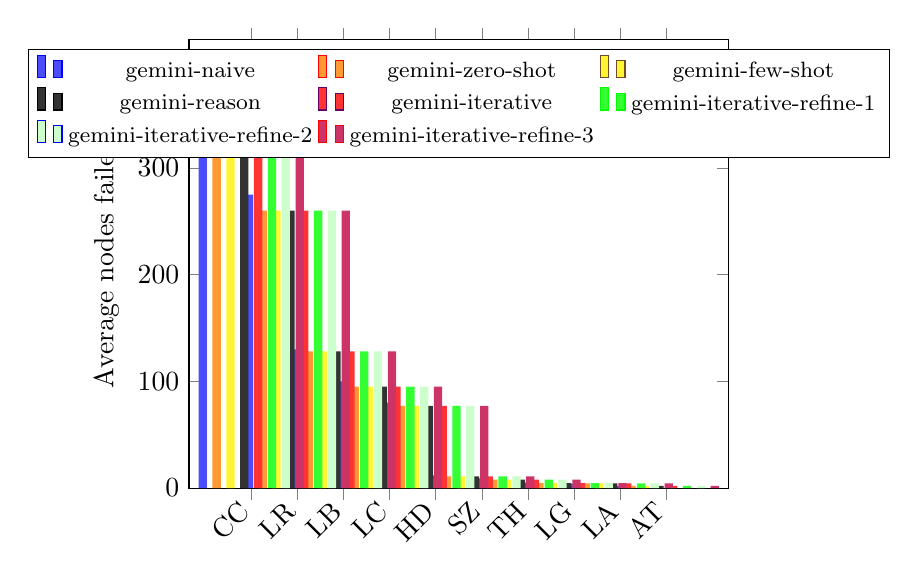
\begin{tikzpicture}
\begin{axis}[
  ybar,
  bar width=3pt,
  ymin=0,   ymax=420,
  symbolic x coords={CC,LR,LB,LC,HD,SZ,TH,LG,LA,AT},
  xtick=data,
  xticklabel style={rotate=45, anchor=east},
  ylabel={Average nodes failed},
  enlarge x limits=0.15,
  legend style={
     font=\footnotesize,
     at={(0.5,0.98)}, anchor=north, legend columns=3},
  every node near coord/.append style={font=\scriptsize}
]
% ----------- DATA SERIES (EXAMPLE VALUES) -----------------
\addplot+[draw=none, fill=blue!70] coordinates {
  (CC,350) (LR,275) (LB,130) (LC,100) (HD,80)
  (SZ,12)  (TH,9)   (LG,5)   (LA,4)   (AT,2)
}; \addlegendentry{gemini-naive}

\addplot+[draw=none, fill=orange!80] coordinates {
  (CC,330) (LR,260) (LB,128) (LC,95)  (HD,77)
  (SZ,11)  (TH,8)   (LG,4.7) (LA,4.3) (AT,2.1)
}; \addlegendentry{gemini-zero-shot}

\addplot+[draw=none, fill=yellow!80] coordinates {
  (CC,330) (LR,260) (LB,128) (LC,95)  (HD,77)
  (SZ,11)  (TH,8)   (LG,4.7) (LA,4.3) (AT,2.1)
}; \addlegendentry{gemini-few-shot}

\addplot+[draw=none, fill=black!80] coordinates {
  (CC,330) (LR,260) (LB,128) (LC,95)  (HD,77)
  (SZ,11)  (TH,8)   (LG,4.7) (LA,4.3) (AT,2.1)
}; \addlegendentry{gemini-reason}

\addplot+[draw=none, fill=red!80] coordinates {
  (CC,330) (LR,260) (LB,128) (LC,95)  (HD,77)
  (SZ,11)  (TH,8)   (LG,4.7) (LA,4.3) (AT,2.1)
}; \addlegendentry{gemini-iterative}

\addplot+[draw=none, fill=green!80] coordinates {
  (CC,330) (LR,260) (LB,128) (LC,95)  (HD,77)
  (SZ,11)  (TH,8)   (LG,4.7) (LA,4.3) (AT,2.1)
}; \addlegendentry{gemini-iterative-refine-1}

\addplot+[draw=none, fill=green!20] coordinates {
  (CC,330) (LR,260) (LB,128) (LC,95)  (HD,77)
  (SZ,11)  (TH,8)   (LG,4.7) (LA,4.3) (AT,2.1)
}; \addlegendentry{gemini-iterative-refine-2}

\addplot+[draw=none, fill=purple!80] coordinates {
  (CC,330) (LR,260) (LB,128) (LC,95)  (HD,77)
  (SZ,11)  (TH,8)   (LG,4.7) (LA,4.3) (AT,2.1)
}; \addlegendentry{gemini-iterative-refine-3}


\end{axis}
\end{tikzpicture}}
\caption{Mean number of WCAG violations per rule group. Abbreviations are explained in Table~\ref{tab:abbr}.}
\label{fig:wcag-fullwidth}
\end{figure*}

% --------------------------------------------------------------------
% 2) EXPLANATORY TABLE FOR THE ABBREVIATIONS
% --------------------------------------------------------------------
\begin{table}[!ht]
\centering
\caption{Mapping of two-letter abbreviations to WCAG rule groups (used in Fig.~\ref{fig:wcag-fullwidth}).}
\label{tab:abbr}
\begin{tabularx}{\linewidth}{@{} l X @{}}
\toprule
\textbf{Abbr.} & \textbf{WCAG rule group} \\
\midrule
CC & Color Contrast: Text \\ 
LR & Landmark \& Region: Missing \& Unique Landmarks \\
LB & Label: Multiple Elements; Content Missing \\
LC & Links: Distinguishable Color \\
HD & Headings: Wrong Order; Empty \& Missing Headings \\
SZ & Size: Target Size; Element Too Small \\
TH & Tables: Table Headers \\
LG & Language: Document Lang Missing / Invalid \\
LA & Links: Missing Descriptive Content of \texttt{<a>} \\
AT & Alt-Text: Images \\
\bottomrule
\end{tabularx}
\end{table}
